\chapter{Gauge Duality Theory}	\label{Sec:PLGD}




\section{Introduction} 	\label{Subsec:PLGD-intro}

This chapter presents the gauge duality theory necessary for optimizing the PLGD model 
\begin{equation*}
\begin{array}{ll}
	\min\limits_{\substack{y}}
					&	\lambda_1(\caA^* y)
						\\
	\st
					&	\langle b, y \rangle - \epsilon ||y||_2 \geq 1.
\end{array}
\end{equation*}
We begin in Section \ref{Subsec:PLGD-models_intro} by stating the PhaseLift primal (PLP) and gauge dual (PLGD) pair of models and reviewing key definitions.
Section \ref{Subsec:PLGD-models_intro} also states a few more general primal-gauge dual model pairs and provides a brief history of gauge duality theory.
In Section \ref{Subsec:PLGD-theory} we prove the gauge duality theorem (Theorem \ref{Thm:P-GD-inequality_pair_are_duals}) for a more general primal-gauge dual model pair and establish weak duality, strong duality, and optimality conditions for this pair.
Section \ref{Subsec:PLGD-opt_conds_primal_recovery} then returns to the PLP-PLGD pair, establishing key properties for optimizing the PLGD model and recovering a signal $x$ from a given dual variable $y$.  

All of the gauge properties and gauge duality results in this chapter were previously established in \cite{rockafellar1970convex}, \cite{DBLP:journals/mp/Freund87}, \cite{DBLP:journals/siamjo/FriedlanderMP14}, and \cite{DBLP:journals/siamsc/FriedlanderM16}.  Gauge functions were first analyzed in  \cite{rockafellar1970convex}.  Gauge duality was then introduced in \cite{DBLP:journals/mp/Freund87}, where the author focused on quadratic programming applications.  
In \cite{DBLP:journals/siamjo/FriedlanderMP14}, the authors developed a broad set of antipolar calculus results for the analysis of gauge duality.  
These results were then applied to the PLP-PLGD pair to develop a first-order method in \cite{DBLP:journals/siamsc/FriedlanderM16}.


Our contribution is to provide a self-contained, comprehensive treatment of gauge duality theory for the PLP-PLGD pair.  
Prior to this treatment, the results in this chapter were spread throughout the original texts ( \hspace{-0.24cm} \cite{rockafellar1970convex}, \cite{DBLP:journals/siamjo/FriedlanderMP14}, and \cite{DBLP:journals/siamsc/FriedlanderM16}), occasionally with differing notation or style.  
In contrast, Section \ref{Subsec:PLGD-models_intro} provides a single notation and style which is used in Sections \ref{Subsec:PLGD-theory} and \ref{Subsec:PLGD-opt_conds_primal_recovery} to develop gauge duality theory for the PLP-PLGD pair.  
The results of this chapter provide the theoretical foundation for developing a first-order optimization method for the PLGD model in Chapter \ref{Sec:PLGD_algo}.


\section{Primal-Gauge Dual Pairs and Definitions}		\label{Subsec:PLGD-models_intro}



The PhaseLift primal semidefinite program (restated from (\ref{Eqn:PhaseLift}) in Section \ref{Subsubsec:phase_retrieval-unstructured}) and its gauge dual are
\begin{equation} \label{Eqn:PhaseLift-P-GD}
\begin{array}{lllllll}
	&	\min\limits_{\substack{X}}
		&	||X||_1 = \sum\limits_{\substack{i=1}}^{\substack{n}} \sigma_i(X)
			&
				&	\min\limits_{\substack{y}}
					&	\lambda_1(\caA^* y)
						\\
\textnormal{(PLP)}
	&	\st
		& 	|| \caA (X) - b ||_2 \leq \epsilon
			&	\hspace{0.4cm} 	\textnormal{(PLGD)}
				&	\st
					&	\langle b, y \rangle - \epsilon ||y||_2 \geq 1.
						\\

	&
		&	X \succeq 0

\end{array}
\end{equation}
This section places the PLP-PLGD pair (\ref{Eqn:PhaseLift-P-GD}) in the context of gauge duality theory.  We begin by discussing definitions and basic properties which are relevant to gauge duality theory. 
We then take a moment to highlight some parallels between gauge duality and Lagrange duality before closing with a summary of major developments in gauge duality theory.  
Along the way, we present three additional, more general primal-gauge dual models which have the PLP-PLGD pair (\ref{Eqn:PhaseLift-P-GD}) as a special case.  Two of these models are then used in Section \ref{Subsec:PLGD-theory} to develop the theory which establishes the gauge duality of the PLP-PLGD pair.




The PLP-PLGD pair (\ref{Eqn:PhaseLift-P-GD}) is an example of a more general primal-gauge dual pair which we define as the \textit{nonlinearly-constrained} pair
\begin{equation} 			\label{Eqn:PhaseLift_P_GD_nonlinear_form}
\begin{array}{lllllll}
	&	\min\limits_{\substack{x \in \caX}}
		&	\kappa(x)
			&
				&	\min\limits_{\substack{z \in \caX}}
					&	\kappa^\circ(z)
						\\
\textnormal{(P-nonlin)}
	&	\st
		& 	x \in \caC
			&	\hspace{3cm} 	\textnormal{(GD-nonlin)}
				&	\st
					&	z \in \caC'.
\end{array}
\end{equation}
Here, $\caC$ and $\caC'$ are subsets of $\caX$, a finite-dimensional Euclidean space.  The set $\caC'$ is the \textit{antipolar} of $\caC$, defined as
\begin{equation}  			\label{Def:antipolar_set}
\caC' = \{ z \ | \ \langle x, z \rangle \geq 1 \ \forall x \in \caC \}.
\end{equation}
This is in contrast to the \textit{polar} of $\caC$, which is defined as
\begin{equation} 			\label{Def:polar}
\caC^\circ = \left\{ z \ | \ \langle x, z \rangle \leq 1 \ \forall x \in \caC \right\}.
\end{equation}
Although we refer to the primal-gauge dual pair (\ref{Eqn:PhaseLift_P_GD_nonlinear_form}) as nonlinear, we are primarily concerned with closed, convex sets $\caC$ which do not contain the origin (e.g., the PLP (\ref{Eqn:PhaseLift-P-GD}) constraint set when $\epsilon < ||b||_2$).  
Note that gauge dual models with linear constraints which do not include the origin are a subset of the models described by (\ref{Eqn:PhaseLift_P_GD_nonlinear_form}).

The functions $\kappa, \kappa^\circ : \caX \rightarrow \bbR \cup \{+\infty\}$ in (\ref{Eqn:PhaseLift_P_GD_nonlinear_form}) are \textit{gauge} functions, meaning they are convex, nonnegative, positively homogeneous ($\kappa(\alpha x) = \alpha \kappa(x)$ for all $\alpha > 0$), and vanish at the origin.  Gauge functions generalize the notion of norms, allowing for flexibility in modeling the phase retrieval problem.  In the PLP model for instance, the Schatten $1$-norm $\kappa(X) := || X ||_1$ and  vector $2$-norm $\rho(y) := ||y||_2$ are both gauges.

Given a gauge function $\kappa$, the \textit{polar} of this function is the function $\kappa^\circ$ that most tightly satisfies the inequality
\begin{equation}  			\label{Def:polar_function_1}
\begin{array}{ll}
	\langle x, z \rangle \leq \kappa(x) \kappa^\circ(z)
			&	\forall x \in \textnormal{dom} \ \kappa, \ \forall z \in \textnormal{dom} \ \kappa^\circ.
\end{array}
\end{equation}
Equivalently, the polar may be defined as \cite[Section 15]{rockafellar1970convex}
\begin{equation}  			\label{Def:polar_function_2}
\kappa^\circ(z) = \inf \left\{ \mu > 0 \ | \ \langle x, z \rangle \leq \mu \kappa(x) \ \forall x \right\}.
\end{equation}
Note that the polar is a generalization of the \textit{dual norm}, which is defined as
\begin{equation}			\label{Def:dual_norm}
||z||_* = \sup_{x} \halfspace \{ \halfspace  \langle x, z \rangle \ | \ ||x|| \leq 1 \}.
\end{equation}
The \textit{preimage} of a linear operator $A: \caX \rightarrow \caY$ over the set $\caS \subseteq \caY$ is defined as 
\begin{equation} 			\label{Def:preimage}
A^{-1} \caS = \{ x \in \caX \ | \ Ax \in \caS \}.
\end{equation}
The \textit{closure} of a set $\caS \subseteq \caX$ is denoted $\textnormal{cl}(\caS)$. The \textit{affine hull} of $\caS$ is the set of all affine combinations of elements of $\caS$, or
\begin{equation}			\label{Def:affine_hull}
\text{aff}(\caS) = \left\{ \sum_{i=1}^k \alpha_i x_i \ \middle| \ k > 0, \ x_i \in \caS, \ \alpha_i \in \bbR, \ \sum_{i=1}^k \alpha_i = 1 \right\}.
\end{equation}
The \textit{relative interior} of $\caS$, denoted $\textnormal{ri}(\caS)$, is the interior within the affine hull of $\caS$, i.e.,
\begin{equation}			\label{Def:relative_interior}
\text{ri}(\caS) = \{ x \in \caS \ | \ \exists \ \epsilon > 0, \ B_\epsilon(x) \cap \text{aff}(\caS) \subseteq \caS  \},
\end{equation}
where $B_\epsilon(x)$ is a ball of radius $\epsilon$ centered at $x$.
The \textit{support} function $\sigma_\caC$ of a nonempty convex set $\caC$ is defined as
\begin{equation}		\label{Def:support_function}
\sigma_\caC(z) = \sup_{x \in \caC} \langle x, z \rangle.
\end{equation}
And the \textit{Minkowski} function $\gamma_\caC$ is defined as
\begin{equation}			\label{Def:Minkowski_function}
\gamma_\caC(x) = \inf \left\{ \lambda \geq 0 \ | \ x \in \lambda \caC  \right\}.
\end{equation}
If there is no $\lambda$ such that $\lambda x \in \caC$, then $\gamma_\caC(x) = + \infty$.  Note that any gauge $\kappa$ is a Minkowski function $\gamma_\caC$ for $\caC = \{ x \ | \ \kappa(x) \leq 1 \}$ \cite[Section 15]{rockafellar1970convex}.  Given a function $f : \caX \rightarrow \bbR \cup \{+\infty\}$, the \textit{epigraph} of $f$ is defined as
\begin{equation}		\label{Eqn:epigraph}
\textnormal{epi}(f) = \left\{ (x, \tau) \ | \ f(x) \leq \tau  \right\}.
\end{equation}
Note that $f$ is convex if and only if $\textnormal{epi}(f)$ is convex \cite[Section 7]{rockafellar1970convex}.  Thus the function $f$ is said to be \textit{closed} if $\textnormal{epi}(f)$ is closed.  Additionally, $f$ is closed if and only if it is lower-semicontinuous (that is, $\liminf_{x \rightarrow x_0} f(x) \geq f(x_0)$ for all $x_0$ in $\textnormal{dom}(f)$) \cite[Section 7]{rockafellar1970convex}.  Also, $f$ is \textit{proper} if the domain of $f$, $\textnormal{dom}(f) = \{ x \ | \ f(x) < +\infty \}$ is nonempty.  

If $\kappa$ is a closed gauge, then its polar may also be expressed as \cite[Section 15]{rockafellar1970convex}
\begin{equation}			\label{Def:polar_function_3}
\kappa^\circ(z) = \sup\limits_x \left\{ \langle x, z \rangle \ | \ \kappa(x) \leq 1 \right\},
\end{equation}
again highlighting the fact that the polar function is a generalization of the dual norm (\ref{Def:dual_norm}).  
Additionally, if $\kappa$ is also positive everywhere except at the origin then its polar may also be defined as \cite[Section 15]{rockafellar1970convex}
\begin{equation}			\label{Def:polar_function_4}
\kappa^\circ(z) = \sup\limits_x \left\{ \frac{\langle x, z \rangle}{\kappa(x)} \right\}.
\end{equation}





Given the gauge duality notation discussed above, we take a moment to contrast gauge duality with the much more common Lagrange duality.  Whereas gauge duality involves multiplicative duality transformations, Lagrange duality is additive in nature.  The reader may see \cite[Chapter 5]{boyd2004convex} for a comprehensive introduction to Lagrange duality, and \cite[Section 28]{rockafellar1970convex} or \cite[Chapter 2]{ben2001lectures} for a treatment of Lagrange duality theory.


Given P-nonlin, the primal model in (\ref{Eqn:PhaseLift_P_GD_nonlinear_form}), we see that its gauge dual GD-nonlin can be stated simply using the polar function $\kappa^\circ$ and the antipolar set $\caC'$.  
Similarly, the Lagrange dual of P-nonlin can be described using the appropriate function and set transformations.  Given a function $f : \caX \rightarrow \bbR \ \cup \ \{\pm \infty\}$, the \textit{convex conjugate} $f^*$ is defined as the function that most tightly satisfies the inequality
\begin{equation} 			\label{Def:conjugate_function_1}
\begin{array}{ll}
	\langle x, z \rangle \leq f(x) + f^*(z)
			&	\forall x \in \textnormal{dom} \ f, \ \forall z \in \textnormal{dom} \ f^*.
\end{array}
\end{equation}
Equivalently, the convex conjugate may be defined as \cite[Section 12]{rockafellar1970convex}
\begin{equation} 			\label{Def:conjugate_function_2}
f^*(z) = \sup_x \left\{ \langle x, z \rangle - f(x)  \right\}.
\end{equation}
We see that (\ref{Def:conjugate_function_1}) and (\ref{Def:conjugate_function_2}) are the additive analogs of the polar function definitions (\ref{Def:polar_function_1}) and (\ref{Def:polar_function_4}), respectively.  Additionally, for a set $\caS \subseteq \caX$, the \textit{dual cone} is defined as
\begin{equation}			\label{Def:dual_cone}
\caS^* = \{ z \ | \ \langle x, z \rangle \leq 0 \ \forall x \in \caS \}.
\end{equation}
Given the convex conjugate $\kappa^*$ and the dual cone $\caC^*$, the Lagrange dual D-nonlin and gauge dual GD-nonlin both have the simple forms
\begin{equation} 			
\begin{array}{lllllll}
	&	\max\limits_{\substack{z}}
		&	-\kappa^*(z)
			&
				&	\min\limits_{\substack{z \in \caX}}
					&	\kappa^\circ(z)
						\\
\textnormal{(D-nonlin)}
	&	\st
		&z \in \caC^*
			&	\hspace{2cm} 	\textnormal{(GD-nonlin)}
				&	\st
					&	z \in \caC'.
\end{array}
\end{equation}
Note that Lagrange duality applies for any function $f : \caX \rightarrow \bbR \ \cup \ \{\pm \infty\}$ and set $\caS \subseteq \caX$.  Thus Lagrange duality has been studied thoroughly and applied extensively (e.g., see \cite[Chapter 5]{boyd2004convex}).  In contrast, gauge duality places specific restrictions on the objective function and constraint set.  As a result,  the development of gauge duality theory has a brief, sporadic history.






In 1970, Rockafellar thoroughly analyzed gauge functions and their polars \cite[Part III]{rockafellar1970convex}.  
The concept of gauge duality was then introduced by Freund in 1987 \cite{DBLP:journals/mp/Freund87}.  
This seminal work focused primarily on the \textit{linearly-constrained} primal and gauge dual pair
\begin{equation} 			\label{Eqn:PhaseLift_P_GD_linear_form}
\begin{array}{lllllll}
	&	\min\limits_{\substack{x \in \caX}}
		&	\kappa(x)
			&
				&	\min\limits_{\substack{y \in \caY}}
					&	\kappa^\circ(A^*y)
						\\
\textnormal{(P-lin)}
	&	\st
		& 	Ax=b
			&	\hspace{3cm} 	\textnormal{(GD-lin)}
				&	\st
					&	\langle b, y \rangle = 1.
\end{array}
\end{equation}
Here $A : \caX \rightarrow \caY$ is a linear operator over finite-dimensional Euclidean spaces. 
As with Lagrange duality, if the primal constraint is replaced with $Ax \geq b$ then the gauge dual also includes the constraint $y \geq 0$.  
Freund develops strong duality and optimality conditions for the pair (\ref{Eqn:PhaseLift_P_GD_linear_form}) based on polarity relationships for sets and gauge functions.  
His work also establishes these conditions for the nonlinear pair (\ref{Eqn:PhaseLift_P_GD_nonlinear_form}).  
In this case, his work requires $\caX$ and $\caY$ to be \textit{ray-like} (meaning that for all $x, y \in \caX$ we have $x + \alpha y \in \caX$ for all $\alpha \geq 0$).  
The addition of the ray-like property to $\caX$ (along with closed, convex, and containing the origin) guarantees $\caX'' = \caX$.


Gauge duality theory was revisited in \cite{DBLP:journals/siamjo/FriedlanderMP14}, where the authors consider the \textit{inequality-constrained} primal and gauge dual pair
\begin{equation} 			\label{Eqn:PhaseLift_P_GD_inequality_form}
\begin{array}{lllllll}
	&	\min\limits_{\substack{x \in \caX}}
		&	\kappa(x)
			&
				&	\min\limits_{\substack{y \in \caY}}
					&	\kappa^\circ(A^*y)
						\\
\textnormal{(P-ineq)}
	&	\st
		& 	\rho(Ax-b) \leq \epsilon
			&	\hspace{0.4cm} 	\textnormal{(GD-ineq)}
				&	\st
					&	\langle b, y \rangle - \epsilon \rho^\circ(y) \geq 1.
\end{array}
\end{equation}
As we will see in Section \ref{Subsec:PLGD-opt_conds_primal_recovery}, the PLP-PLGD pair (\ref{Eqn:PhaseLift-P-GD}) pair is recovered from (\ref{Eqn:PhaseLift_P_GD_inequality_form}) when we set $\kappa(X) = ||X||_1 + \delta_{(\cdot) \succeq 0}(X)$ and $\rho(y) = ||y||_2$.  The authors of \cite{DBLP:journals/siamjo/FriedlanderMP14} develop an antipolar calculus to determine the antipolar for sets like $\{ y \ | \ \rho(Ax-b) \leq \epsilon \}$ and use this calculus rather than polarity relations to derive the gauge dual pair (\ref{Eqn:PhaseLift_P_GD_inequality_form}) and establish conditions such as those for strong duality.  Additionally, this antipolar calculus allows the authors to drop the requirement that the sets $\caX$ and $\caY$ are ray-like.

In contrast to the antipolar calculus framework, the authors of \cite{aravkin2017foundations} develop gauge duality through a perturbation framework.  This even broader setting frames gauge duality as a product of Fenchel-Rockafellar duality, allowing the consideration of gauge duality for 
general nonnegative convex functions.









\section{The Gauge Duality Theorem and Optimality Conditions} 			\label{Subsec:PLGD-theory}




In this section we develop gauge duality theory for the inequality-constrained primal and gauge dual pair (\ref{Eqn:PhaseLift_P_GD_inequality_form}).  
We begin by establishing the propositions necessary to show the gauge duality of (\ref{Eqn:PhaseLift_P_GD_inequality_form}) is a consequence of the duality of both the nonlinear (\ref{Eqn:PhaseLift_P_GD_nonlinear_form}) and linear (\ref{Eqn:PhaseLift_P_GD_linear_form}) pairs.  
This two-track proof strategy as depicted in Figure \ref{Fig:gauge_duality_thm_flowchart} leads to Theorem \ref{Thm:P-GD-inequality_pair_are_duals}, (i) and (ii), respectively.
\begin{figure}[H] 
\centering
\hspace{0cm}
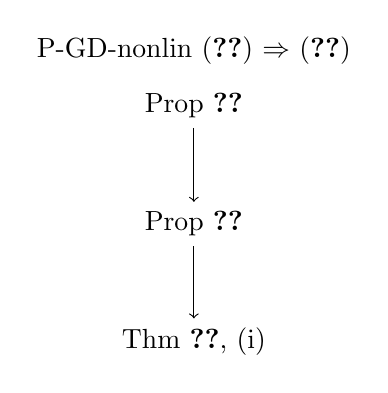
\begin{tikzpicture} 
	\node (1) at (0,3.7) {P-GD-nonlin (\ref{Eqn:PhaseLift_P_GD_nonlinear_form}) $\Rightarrow$ (\ref{Eqn:PhaseLift_P_GD_inequality_form})};
 	\node (2) at (0,3) {Prop \ref{Prop:antipolar_set_equalities}};
	\node (3) at (0,1.5) {Prop \ref{Prop:antipolar_of_primal_phase_retrieval}};
	\node (4) at (0,0) {Thm \ref{Thm:P-GD-inequality_pair_are_duals}, (i)};
	\draw[->] (2) -- (3);
	\draw[->] (3) -- (4);
\end{tikzpicture}
\hspace{1cm}
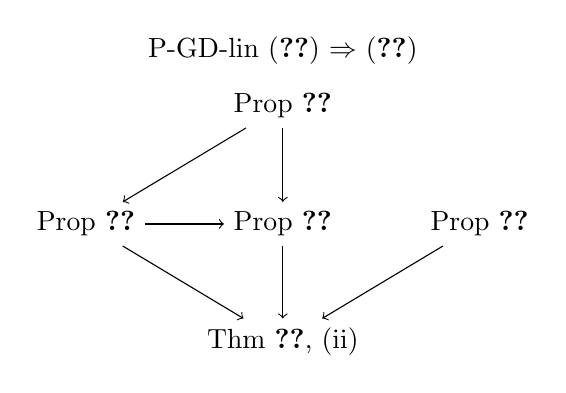
\begin{tikzpicture}
	\node (6) at (2.5,3.7) {P-GD-lin (\ref{Eqn:PhaseLift_P_GD_linear_form}) $\Rightarrow$ (\ref{Eqn:PhaseLift_P_GD_inequality_form})};
	\node (1) at (2.5,3) {Prop \ref{Prop:P-GD-Minkowski_set_unique}};
	\node (2) at (0,1.5) {Prop \ref{Prop:P-GD-polar_of_sum_of_gauges_sets_equal}};
	\node (3) at (2.5,1.5) {Prop \ref{Prop:P-GD-polar_of_sum_of_gauges}};
	\node (4) at (5,1.5) {Prop \ref{Prop:P-GD-indicator_epigraph_polar}};
	\node (5) at (2.5,0) {Thm \ref{Thm:P-GD-inequality_pair_are_duals}, (ii)};
	\draw[->] (1) -- (2);
	\draw[->] (1) -- (3);
	\draw[->] (2) -- (3);
	\draw[->] (2) -- (5);
	\draw[->] (3) -- (5);
	\draw[->] (4) -- (5);
\end{tikzpicture}
\caption{Dependency chart for proofs (i) and (ii) of Theorem \ref{Thm:P-GD-inequality_pair_are_duals} which establish the gauge duality of P-GD-ineq (\ref{Eqn:PhaseLift_P_GD_inequality_form}).
  	}
\label{Fig:gauge_duality_thm_flowchart}
\end{figure}

Following Theorem \ref{Thm:P-GD-inequality_pair_are_duals} we establish weak duality, strong duality, and optimality conditions for (\ref{Eqn:PhaseLift_P_GD_inequality_form}).  In Section \ref{Subsec:PLGD-opt_conds_primal_recovery} we will return to the PhaseLift model (\ref{Eqn:PhaseLift-P-GD}), where the optimality conditions in this section provide a method for recovery of a primal signal $x$ from a dual variable $y$.


The results in this section are based on \cite{rockafellar1970convex}, \cite{DBLP:journals/mp/Freund87}, and especially \cite{DBLP:journals/siamjo/FriedlanderMP14}, and rely on the analysis of polarity relations rather than perturbation analysis as discussed in \cite{aravkin2017foundations}.    
In particular, the two-track proof strategy depicted in Figure \ref{Fig:gauge_duality_thm_flowchart} was first developed in \cite{DBLP:journals/siamjo/FriedlanderMP14} as part of a larger treatment of antipolar calculus and the authors referred to \cite{rockafellar1970convex} for more elementary results. 
This section provides a self-contained development of gauge duality for (\ref{Eqn:PhaseLift_P_GD_inequality_form}).





The next two propositions are used in Theorem \ref{Thm:P-GD-inequality_pair_are_duals}, (i) to show the inequality pair (\ref{Eqn:PhaseLift_P_GD_inequality_form}) is an instance of the nonlinear pair (\ref{Eqn:PhaseLift_P_GD_nonlinear_form}).  Since (\ref{Eqn:PhaseLift_P_GD_inequality_form}) allows for the constraint set $\caC$ to be any closed, convex set not containing the origin, we must simply establish the antipolar of the constraint set $\caC = \{ x \ | \rho(Ax-b) \leq \epsilon\}$.  We begin by showing how linear and polar transformations on $\caC$ commute under certain assumptions.





\begin{prop}		\label{Prop:antipolar_set_equalities}
Let $\caX$ and $\caY$ be finite-dimensional Euclidean spaces, $\caC \subseteq \caX$ a closed, convex set which does not contain the origin, $A : \caX \rightarrow \caY$ a linear operator, and $A^* : \caY \rightarrow \caX$ its adjoint.
%(so $\langle A^*y, x\rangle = \langle y, Ax \rangle$ for all $x \in \caX$ and $y \in \caY$).    
Then
\begin{equation}		\label{Eqn:antipolar_set_equalities_1}
\begin{array}{rll}
\left( A \caC \right)' & = & 	\left( A^* \right)^{-1} \caC' .
\end{array}
\end{equation}

Additionally, assume $\caC$ is polyhedral or $\textnormal{ri}(\caC) \cap \textnormal{range}(A) \neq \emptyset$, and $A^{-1}\caC$ is not empty.  
Then $( A^{-1} \caC)'$ is nonempty and the following set equality holds
% (A\caC)'	&	=	&	\left( A^* \right)^{-1} \caC'	\\
\begin{equation}		\label{Eqn:antipolar_set_equalities_2}
\begin{array}{rll}
\left( A^{-1} \caC \right)' & = &  A^* \caC' .
\end{array}
\end{equation}
\end{prop}
\begin{proof}
The first result is proved in \cite[Proposition 3.3]{DBLP:journals/siamjo/FriedlanderMP14} and the second in \cite[Proposition 3.4, 3.5]{DBLP:journals/siamjo/FriedlanderMP14}.
\end{proof}


The previous propositions allows us to construct the antipolar of the constraint set $\caC = \{ x \ | \ \rho(Ax-b) \leq \epsilon \}$ in Proposition \ref{Prop:antipolar_of_primal_phase_retrieval}.

\begin{prop}		\label{Prop:antipolar_of_primal_phase_retrieval}
Let $\caX$ and $\caY$ be finite-dimensional Euclidean spaces, $A : \caX \rightarrow \caY$ a linear operator, and $A^* : \caY \rightarrow \caX$ its adjoint.  Let $\caC = \{ x \ | \ \rho(Ax-b) \leq \epsilon \}$ with $0 < \epsilon < \rho(b)$.  Also assume $\textnormal{ri}(\caC) \cap \textnormal{range}(A)$ and $A^{-1}\caC$ are not empty. Then
\begin{equation}			\label{Eqn:antipolar_of_primal_phase_retrieval}
\caC' = \left\{ A^*y \ | \ \langle b, y \rangle - \epsilon \rho^\circ(y) \geq 1  \right\}.	
\end{equation}
\end{prop}
\begin{proof}
Since the arguments of $\rho$ lie in $\caY$, we first consider the antipolar of $\caD = A\caC \subseteq \caY$ to establish the constraint $\langle b, y \rangle - \epsilon \rho^\circ(y) \geq 1$.  Note that $y \in \caD'$ is equivalent to $\langle Ax, y \rangle \geq 1$ for all $Ax \in A\caC$.  This is again equivalent to
\begin{equation}				\label{Eqn:antipolar_eqn_for_proof_1}
\langle b - Ax, y \rangle \leq \langle b, y \rangle - 1 \ \forall x \ \textnormal{such that} \ \rho(Ax-b) \leq \epsilon.
\end{equation}
Next apply definition (\ref{Def:polar_function_3}) for the antipolar $\rho^\circ$ and take the supremum over $u = \frac{b-Ax}{\epsilon}$, giving 
\begin{equation}  		\label{Eqn:antipolar_eqn_for_proof_2}
\begin{array}{lll}
\epsilon \rho^\circ(y) 	&	=	&	\epsilon \sup\limits_{\substack{u}} \left\{ \langle u, y \rangle \ | \ \rho(u) \leq 1, \ u = \frac{b-Ax}{\epsilon}  \right\} 	\\
	&	= 	&  \sup\limits_{\substack{x}} \left\{ \langle b - Ax, y \rangle \ | \ \rho\left(\frac{b-Ax}{\epsilon}\right) \leq 1  \right\} \\
		&	= 	&  \sup\limits_{\substack{x}} \left\{ \langle b - Ax, y \rangle \ | \ \rho(b-Ax) \leq \epsilon  \right\},
\end{array}
\end{equation}
where the last equality uses the postive homogeneity of the gauge $\rho$.  Using equation (\ref{Eqn:antipolar_eqn_for_proof_2}), we see that equation (\ref{Eqn:antipolar_eqn_for_proof_1}) is equivalent to the desired constraint $\epsilon \rho^\circ(y) \leq  \langle b, y \rangle - 1$.  Thus $\caD' = \{ y \ | \ \langle b, y \rangle - \epsilon \rho^\circ(y) \geq 1 \}$.

Finally, note that $\caC$ and $\caC'$ both lie in $\caX$, while $\caD = A\caC$ and $\caD'$ lie in $\caY$.  Then by Proposition \ref{Prop:antipolar_set_equalities}, the antipolar $\caC'$ has the form
\begin{equation}
\begin{array}{lll}
\caC' = \left(A^{-1} \caD \right)'	& =  &	A^* \caD' 	\\
	&	=	&		\left\{ A^*y 	\	|	\ \langle b, y \rangle - \epsilon \rho^\circ(y) \geq 1  \right\}.
\end{array}
\end{equation}
\end{proof}





The next four propositions allow us to derive the inequality-constrained primal-gauge dual pair (\ref{Eqn:PhaseLift_P_GD_inequality_form}) from the linearly-constrained pair (\ref{Eqn:PhaseLift_P_GD_linear_form}) by transforming the P-ineq model into a linearly-constrained gauge model of the form P-lin (see the dependency map in Figure \ref{Fig:gauge_duality_thm_flowchart} for reference).   
This process uses an indicator function to embed the constraint set $\caC = \{ x \ | \ \rho(Ax-b) \leq \epsilon\}$ into the primal objective function, resulting in a P-lin model (\ref{Eqn:PhaseLift_P_GD_linear_form}).  Finally, we determine the gauge dual of the resulting model using polar relations and properties established in Section \ref{Subsec:PLGD-models_intro}.


The first two propositions show that we may discuss the polar of a sum of gauges in terms of sets induced by Minkowski functions.  This allows us to determine the polar of a sum of gauges in Proposition \ref{Prop:P-GD-polar_of_sum_of_gauges}.

\begin{prop} 			\label{Prop:P-GD-Minkowski_set_unique}
Let $\caC \subseteq \caX$ be a closed, convex set containing the origin and $\kappa = \gamma_\caC$ the Minkowski function induced by $\caC$.  Then $\kappa$ is a gauge, $\caC = \{ x \ | \ \kappa(x) \leq 1 \}$, and $\caC$ is the unique closed, convex set containing the origin such that $\kappa = \gamma_\caC$.
\end{prop}
\begin{proof}
To verify that $\kappa$ is a gauge, first note that positive homogeneity and $\kappa(0) = 0$ are direct results of $\kappa$ being a Minkowski function.  To show convexity, let $x, y \in \caX$ and $0 \leq \alpha \leq 1$.  Then $x \in \kappa(x) \caC$ means $\alpha x \in \alpha \kappa(x) \caC$, and likewise $(1-\alpha) y \in (1-\alpha) \kappa(y) \caC$.  Thus $\alpha x + (1-\alpha)y \in (\alpha \kappa(x) + (1-\alpha) \kappa(y)) \caC$.  Then by the infimum of the Minkowski function, $\kappa(\alpha x + (1-\alpha) y) \leq \alpha \kappa(x) + (1-\alpha) \kappa(y)$ and $\kappa$ is convex.

Additionally, $\kappa(x) \leq 1$ is equivalent to $x \in \caC$, and thus $\caC =  \{ x \ | \ \kappa(x) \leq 1 \}$.

Finally, assume there is some closed, convex set $\caD \subseteq \caX$ such that $\kappa = \gamma_\caD$.  Then $\kappa(x) = \gamma_\caC(x) = \gamma_\caD(x) \leq 1$ is equivalent to $x$ being in both $\caC$ and $\caD$, since both sets are closed and convex. Likewise, $\kappa(x) > 1$ indicates $x$ is in neither set.  Thus $\caC = \caD$.

\end{proof}

\begin{prop} 			\label{Prop:P-GD-polar_of_sum_of_gauges_sets_equal}
Let $\kappa_1$ and $\kappa_2$ be gauges.  Let $\kappa(x_1, x_2) = \kappa_1(x_1) + \kappa_2(x_2)$, $\caC_1 = \{ z_1 \ | \ \kappa^\circ(z_1) \leq 1 \}$, $\caC_2 = \{ z_2 \ | \ \kappa^\circ(z_2) \leq 1 \}$, and $\caC = \{ (z_1, z_2) \ | \ \kappa^\circ(z_1, z_2) \leq 1 \}$. Then $\kappa$ and $\kappa^\circ$ are gauges, $\kappa^\circ = \gamma_\caC$, and $\caC = \caC_1 \times \caC_2$.
\end{prop}
\begin{proof}
Since $\kappa$ is the sum of gauges, it is also convex, nonnegative, positively homogeneous, and zero at the origin, and thus a gauge.  Then $\kappa^\circ$ is also a gauge and by Proposition \ref{Prop:P-GD-Minkowski_set_unique}, $\caC$ is the unique set such that $\kappa = \gamma_\caC$.
If $(z_1, z_2) \in \caC$, then $\langle x_1, z_1 \rangle + \langle x_2, z_2 \rangle \leq \kappa(x_1,x_2)\kappa^\circ(z_1,z_2) \leq  \kappa_1(x_1) + \kappa_2 (x_2)$ for all $x_1 \in \textnormal{dom}\ \kappa_1$ and $x_2 \in \textnormal{dom} \ \kappa_2$.  In particular, if $x_2 = 0$ then $\langle x_1, z_1 \rangle \leq \kappa_1(x_1)$ for all $x_1  \in \textnormal{dom}\ \kappa_1$, indicating $z_1 \in \caC_1$.  Similarly $z_2 \in \caC_2$ and thus $\caC_1 \times \caC_2 \subseteq \caC$.  For the reverse inclusion, $(z_1, z_2) \in \caC_1 \times \caC_2$ means $\langle x_1, z_1 \rangle \leq \kappa_1(x_1)$ for all $x_1 \in \textnormal{dom}\ \kappa_1$ and $\langle x_2, z_2 \rangle \leq \kappa_2(x_2)$ for all $x_2 \in \textnormal{dom}\ \kappa_2$.  Adding these inequalities, we have $\langle x_1, z_1 \rangle + \langle x_2, z_2 \rangle \leq \kappa_1(x_1) + \kappa_2 (x_2)$ for all $x_1 \in \textnormal{dom}\ \kappa_1$ and $x_2  \in \textnormal{dom}\ \kappa_2$, and thus $\caC = \caC_1 \times \caC_2$.
\end{proof}


Given the two propositions above, we now show that the polar of a sum of gauges is the max of the set of polars.

\begin{prop}			\label{Prop:P-GD-polar_of_sum_of_gauges}
Let $\kappa_1$ and $\kappa_2$ be gauges.  Then the sum $\kappa(x_1, x_2) := \kappa_1(x_1) + \kappa_2(x_2)$ is a guage and has the polar
\begin{equation}			\label{Eqn:polar_of_sum_of_gauges}
\kappa^\circ(z_1, z_2) = \max \left\{ \halfspace \kappa^\circ(z_1), \ \kappa_2^\circ(z_2) \right\}.
\end{equation}
\end{prop}
\begin{proof}
Proposition \ref{Prop:P-GD-polar_of_sum_of_gauges_sets_equal} shows $\kappa$ and its polar $\kappa^\circ$ are gauges.  Setting $\caC_1 = \{ z_1 \ | \ \kappa^\circ(z_1) \leq 1 \}$, $\caC_2 = \{ z_2 \ | \ \kappa^\circ(z_2) \leq 1 \}$, and $\caC = \{ (z_1, z_2) \ | \ \kappa^\circ(z_1, z_2) \leq 1 \}$, we may express the gauge polars as Minkowski functions $\kappa_1^\circ = \gamma_{\caC_1}$, $\kappa_2^\circ = \gamma_{\caC_2}$, and $\kappa^\circ = \gamma_{\caC}$.  
Since $\caC_1$, $\caC_2$, and $\caC$ are closed, convex sets containing the origin, Proposition \ref{Prop:P-GD-Minkowski_set_unique} tells us these are the unique sets defining $\kappa_1^\circ$, $\kappa_2^\circ$, and $\kappa^\circ$.  Additionally, Proposition \ref{Prop:P-GD-polar_of_sum_of_gauges_sets_equal} implies $\caC = \caC_1 \times \caC_2$ and $\kappa^\circ(z_1, z_2) =	\gamma_{\caC}(z_1, z_2) 	=	\gamma_{\caC_1 \times \caC_2}(z_1, z_2)$.


Then we have
\begin{equation}
\begin{array}{rll}
\kappa^\circ(z_1, z_2)	  & =	&	\gamma_{\caC_1 \times \caC_2}(z_1, z_2)	\\
	&	=	&	\inf \left\{ \halfspace \lambda \geq 0 \ | \ z_1 \in \lambda \caC_1, \ z_2 \in \lambda \caC_2 \right\} \\
	&	=	&	\max \left\{ \halfspace \inf \{ \lambda \geq 0 \ | \ z_1 \in \lambda \caC_1 \}, 
									\ \inf \{ \lambda \geq 0 \ | \ z_2 \in \lambda \caC_2 \} 	\right\}	\\
	&	=	&	\max \left\{ \halfspace \gamma_{\caC_1}(z_1), \ \gamma_{\caC_1}(z_2) \right\}	\\
	&	=	&	\max \left\{ \halfspace \kappa_1^\circ(z_1), \ \kappa_2^\circ(z_2) \right\}.
\end{array}
\end{equation}
\end{proof}


The following proposition establishes two equalities which allow us to compute the polar of an objective function which includes an indicator function.  This strategy allows us to embed the inequality $\rho(Ax-b) \leq \epsilon$ from (\ref{Eqn:PhaseLift_P_GD_inequality_form}) into the objective function of (\ref{Eqn:PhaseLift_P_GD_linear_form}) in the proof of Theorem \ref{Thm:P-GD-inequality_pair_are_duals}, (ii).


\begin{prop}				\label{Prop:P-GD-indicator_epigraph_polar}
Let $\rho$ be a gauge.  Then for all $y \in \caX$ and $\tau \geq 0$ the following equalities hold.
\begin{enumerate}[(i)]
\item
 $\left( \delta_{\textnormal{epi} \halfspace \rho} \right)^\circ(y, \tau) = \delta_{\left(  \textnormal{epi} \halfspace \rho \right)^\circ} (y, \tau)$,
\item
$\delta_{\left( \epi \halfspace \rho \right)^\circ} (y, \tau) = \delta_{\epi \left( \rho^\circ \right)}(y, -\tau)$.
\end{enumerate}
\end{prop}
\begin{proof}
To show (i) holds, consider the expansion of the expressions
\begin{equation*}
\begin{array}{rll}
\left( \delta_{\textnormal{epi} \halfspace \rho} \right)^\circ(y, \tau) 
	&	= 
			&	 \inf \left\{ \mu > 0 \ | \ \langle (x, \sigma), (y, \tau) \rangle \leq \mu \delta_{\epi \halfspace \rho}(x, \sigma) \ \ \forall (x, \sigma) \right\},
					\\
\delta_{\left( \epi \halfspace \rho \right)^\circ} (y, \tau) 
	&	= 
			&	\begin{cases}
						0 	&\textnormal{if } \langle (x, \sigma) , (y, \tau) \rangle \leq 1 \ \ \forall (x, \sigma) \in \epi \halfspace \rho \\
						+\infty	&\textnormal{else}.
				\end{cases}	
\end{array}
\end{equation*}
Note that the value of $\delta_{\left(  \textnormal{epi} \halfspace \rho \right)^\circ} (y, \tau)$ is either $0$ or $+\infty$.  If $\delta_{\left(  \textnormal{epi} \halfspace \rho \right)^\circ} (y, \tau) = 0$, then $\langle (x, \sigma), (y, \tau) \rangle  \leq 1$ for all $(x, \sigma) \in \epi \halfspace \rho$.  Since $\rho$ is a gauge, $(x, \sigma) \in \epi \halfspace \rho$ is equivalent to $\rho(\alpha x) \leq \alpha \sigma$ for all $\alpha > 0$.  Then $(\alpha x, \alpha \sigma) \in \epi \halfspace \rho$ for all $\alpha > 0$.  Dividing the inequality by $\alpha$ and letting $\alpha$ approach infinity, we have
\begin{equation*}
\langle (x, \sigma), (y, \tau) \rangle \leq \lim\limits_{\substack{\alpha \rightarrow +\infty}} \frac{1}{\alpha} = 0 \ \ \textnormal{for all} \ (x, \alpha) \in \epi \halfspace \rho.
\end{equation*}
Thus $\left( \delta_{\textnormal{epi} \halfspace \rho} \right)^\circ(y, \tau)  = 0$.  On the other hand, if $\delta_{\left(  \textnormal{epi} \halfspace \rho \right)^\circ} (y, \tau) = +\infty$ then there is some $(x, \sigma) \in \epi \halfspace \rho$ with $\langle (x, \sigma) , (y, \tau) \rangle > 1$.  Then $\delta_{\epi \halfspace \rho}(x, \sigma) = 0$ and there is no $\mu >0$ such that $\langle (x, \sigma), (y, \tau) \rangle \leq \mu \delta_{\epi \halfspace \rho}(x, \sigma)$.  Thus $\left( \delta_{\textnormal{epi} \halfspace \rho} \right)^\circ(y, \tau)  = +\infty$.

To show (ii) holds, we have the following set of equivalences
\begin{equation*}
\begin{array}{rll}
(y, \tau) \in \left( \epi \halfspace \rho \right)^\circ
	&	\iff	&  \langle (x, \sigma), (y, \tau) \rangle \leq 1 \ \ \forall (x, \sigma) \in  \epi (\rho)
			\\
	&	\iff	&	 \langle (x, \sigma), (y, \tau) \rangle \leq 0 \ \ \forall x \text{ and } \rho(x) \leq \sigma
			\\
	&	\iff	&	\langle x, y \rangle \leq -\tau \rho(x) \ \ \forall x
			\\
	&	\iff	&	\rho^\circ(y) = \inf \left\{ \mu > 0 \ | \ \langle x, y \rangle \leq \mu \rho(x) \ \ \forall x \right\} \leq - \tau
			\\
		&	\iff	&	(y, -\tau)  \in \epi (\rho^\circ).
\end{array}
\end{equation*}
Here, the second equivalence was established in the proof of (i) and the third comes from setting $\sigma$ as the minimal value $\sigma = \rho(x)$.  Thus $\delta_{\left( \epi \halfspace \rho \right)^\circ} (y, \tau) = \delta_{\epi \left( \rho^\circ \right)}(y, -\tau)$.
\end{proof}





We are now prepared to prove the essential results which underly our phase retrieval method and signal recovery strategy.  We begin with the following gauge duality result.

\begin{theorem} 				\label{Thm:P-GD-inequality_pair_are_duals}
Let P-ineq and GD-ineq be the inequality-constrained pair of models from (\ref{Eqn:PhaseLift_P_GD_inequality_form}).  Also let $\caC = \{ x \ | \ \rho(Ax-b) \leq \epsilon \}$ with $0 < \epsilon < \rho(b)$ and assume $\textnormal{ri}(\caC) \cap \textnormal{range}(A)$ and $A^{-1}\caC$ are not empty.  Then the model GD-ineq is the gauge dual of the primal P-ineq based on the gauge duality of 
\begin{enumerate}[(i)]
\item
the nonlinear gauge dual pair (\ref{Eqn:PhaseLift_P_GD_nonlinear_form}), and
\item
the linear gauge dual pair (\ref{Eqn:PhaseLift_P_GD_linear_form}).
\end{enumerate}
\end{theorem}


\begin{proof}
Item (i) is a direct result of Proposition \ref{Prop:antipolar_of_primal_phase_retrieval}, which gives the antipolar set $\caC' = \left\{ A^*y \ | \ \langle b, y \rangle - \epsilon \rho^\circ(y) \geq 1  \right\}$.  As a result, the argument of the GD-nonlin objective $\kappa^\circ$ is $A^*y$ and GD-ineq is equivalent to GD-nonlin.

To prove item (ii), we must first express P-ineq as a linear gauge model of the form P-lin.  Define the function $\phi(x, r, \sigma) = \kappa(x) + \delta_{\epi \halfspace \rho}(r, \sigma)$.  Since the epigraph of a gauge is closed under positive scaling, the indicator function $\delta_{\epi \halfspace \rho}$ is a gauge.  By Proposition \ref{Prop:P-GD-polar_of_sum_of_gauges_sets_equal}, $\phi$ is a gauge, and thus P-ineq is equivalent to the linear gauge model
\begin{equation}   			\label{Eqn:P-GD-Thm_duals-eqn1}
\begin{array}{rl}
\min\limits_{\substack{x, r, \sigma}} 
	&	\phi(x, r, \sigma)	\\
\st
	&	r = b-Ax \\
	&	\sigma = \epsilon.
\end{array}
\end{equation}
To combine these linear constraints, define the following extended matrix and vectors
\begin{equation}
\begin{array}{lll}
\overline{A}
=	\begin{bmatrix}
		A	&	I	&	0	\\
		0	&	0	&	1
	\end{bmatrix},
	&	\overline{x} = \begin{bmatrix}
									x \\ r \\ \sigma
								\end{bmatrix},
	&	\overline{b}	=	\begin{bmatrix}
									b	\\	 \epsilon
								\end{bmatrix},
\end{array}	
\end{equation}
and define the spaces $\overline{\caX} = \caX \times \caY \times \{\bbR \cup +\infty\}$ and $\overline{\caY} = \caY \times \{\bbR \cup +\infty\}$.

Then (\ref{Eqn:P-GD-Thm_duals-eqn1}) has the linear form equivalent to P-lin
\begin{equation}
\begin{array}{rl}
\min\limits_{\substack{\overline{x} \in \overline{\caX}}} \phi(\overline{x})
	&	\st \ \ \overline{A}\overline{x} = \overline{b}.
\end{array}
\end{equation}
This model has the following gauge dual per (\ref{Eqn:PhaseLift_P_GD_linear_form})
\begin{equation}
\begin{array}{rl}
\min\limits_{\substack{\overline{y} \in \overline{\caY}}} \phi^\circ(\overline{A}^*\overline{y})
	&	\st \ \ \langle \overline{b}, \overline{y} \rangle = 1,
\end{array}
\end{equation}
where $\overline{A}^*\overline{y} = (A^*y, y, \tau)$ and $\langle \overline{b}, \overline{y} \rangle = \langle b, y \rangle + \sigma \tau$.

Taking the polar of $\phi$, we have
\begin{equation}
\begin{array}{rcl}
\phi^\circ(A^*y, y, \tau)
	&	=	&	\max \halfspace \{ \halfspace \kappa^\circ(A^*y), \ \left( \delta_{\epi \halfspace \rho} \right)^\circ(y, \tau) \}	\\
	&	=	&	\max \halfspace \{ \halfspace \kappa^\circ(A^*y), \ \delta_{\left( \epi \halfspace \rho \right)^\circ} (y, \tau) \}	\\
	&	=	&	\kappa^\circ(A^*y) + \delta_{\left( \epi \halfspace \rho \right)^\circ}(y, \tau) \\
	&	=	&	\kappa^\circ(A^*y) + \delta_{\epi \left( \rho^\circ \right)} (y, -\tau).
\end{array}
\end{equation}
The first equality is a result of Proposition \ref{Prop:P-GD-polar_of_sum_of_gauges}. The second and last equalities are results of Proposition \ref{Prop:P-GD-indicator_epigraph_polar}, (i) and (ii), respectively.  And the third equality is a consequence of the indicator function mapping to $\{0, +\infty \}$.  

The indicator function $\delta_{\epi \left( \rho^\circ \right)} (y, -\tau)$ corresponds to the constraint $\rho^\circ(y) \leq - \tau$.  This constraint and the equality constraint $\langle b, y \rangle + \sigma \tau = 1$ may be combined as
\begin{equation*}
\langle b, y \rangle - \sigma \rho^\circ(y) \geq \langle b, y \rangle + \sigma \tau = 1.
\end{equation*}
Thus we eliminate $\tau$ and recover GD-ineq.
\end{proof}





With the gauge duality of (\ref{Eqn:PhaseLift_P_GD_inequality_form}) established, we proceed by establishing weak duality, strong duality, and optimality conditions for this pair of models.  These properties will play a central role in the first-order method for optimizing the PLGD model (\ref{Eqn:PhaseLift-P-GD}), allowing us to develop termination conditions as well as a recovery method for the primal signal $x$ from a dual iterate $y$.  The weak duality property of (\ref{Eqn:PhaseLift_P_GD_inequality_form}) is a straightforward consequence of the definition of the polar of a function and inequality constraints in this model.

\begin{prop} \label{Prop:weak_duality}
\emph{(weak duality)}
Assume the primal model P-ineq in (\ref{Eqn:PhaseLift_P_GD_inequality_form}) is feasible and $0 \leq \epsilon < \rho(b)$.  Then for all primal and gauge dual feasible pairs $(x, y) \in \caX \times \caY$ we have
\begin{equation}				\label{Eqn:weak_duality}
\kappa(x) \kappa^\circ ( \caA^* y ) \geq 1.
\end{equation}

\end{prop}
\begin{proof}
Since $x$ and $y$ are feasible for (\ref{Eqn:PhaseLift_P_GD_inequality_form}), we have
\begin{equation} 		\label{Eqn:weak_duality_inequalities}
\begin{array}{rcl}
1 
	&	\leq 	&	\langle b, y \rangle - \epsilon \rho^\circ(y)	\\
	&	\leq 	&	\langle b, y \rangle - \rho(b - Ax) \rho^\circ(y) \\
	&	\leq 	&	\langle b, y \rangle - \langle b - Ax, y \rangle \\
	&	=		&	\langle x, A^*y \rangle \\	
	&	\leq 	&	\kappa(x) \kappa^\circ(A^*y).
\end{array}
\end{equation}
Here, the first and second inequalities are due to GD-ineq and P-ineq feasibility, respectively.  The third and fourth inequalities are a consequence of polar functions.
\end{proof}




In order to show strong duality holds for the pair (\ref{Eqn:PhaseLift_P_GD_inequality_form}), we add the assumption that $\rho^\circ$ is continuous and use the strong duality properties of the Lagrange primal and dual pair (see \cite[Section 28]{rockafellar1970convex})
\begin{equation}			\label{Eqn:PhaseLift_P_GD_ineq_Lagrange_dual}
\begin{array}{lllllll}
	&	\min\limits_{\substack{x \in \caX}}
		&	\kappa(x)
			&
				&	\max\limits_{\substack{y \in \caY}}
					&	\langle b, y \rangle - \epsilon \rho^\circ(y)
						\\
\textnormal{(P-ineq)}
	&	\st
		& 	\rho(Ax-b) \leq \epsilon
			&	\hspace{0.4cm} 	\textnormal{(LD-ineq)}
				&	\st
					&	\kappa^\circ(A^*y)  \leq 1.
\end{array}
\end{equation}
This proof strategy identifies a sequence of Lagrange dual feasible vectors which may be rescaled to create to a gauge dual feasible sequence.
To guarantee the limit of this sequence exists, we require that $\rho^\circ$ is continuous.


\begin{prop} \label{Prop:strong_duality}
\emph{(strong duality)}
Assume the primal model P-ineq in (\ref{Eqn:PhaseLift_P_GD_inequality_form}) is feasible, $\rho^\circ$ is continuous, and $0 \leq \epsilon < \rho(b)$.  Then P-ineq admits an optimal variable $x_\star$ and
\begin{equation} 			\label{Eqn:strong_duality_1}
\kappa(x_\star) \nu_{GD} = 1
\end{equation}
where $\nu_{GD}$ is the optimal GD-ineq value
\begin{equation}
\nu_{GD} := \inf\limits_{\substack{ \langle b, y \rangle - \epsilon \rho^\circ(y) \geq 1}} \kappa^\circ(A^*y).
\end{equation}

Additionally, if P-ineq is strictly feasible then P-ineq and GD-ineq admit an optimal pair $(x_\star, y_\star) \in \caX \times \caY$ and
\begin{equation} 			\label{Eqn:strong_duality_2}
\kappa(x_\star) \kappa^\circ ( \caA^* y_\star ) = 1,
\end{equation}
where $y_\star$ is a rescaling of the optimal LD-ineq variable $\hat{y}$ such that
\begin{equation} 			\label{Eqn:strong_duality_3}
y_\star = \frac{\hat{y}}{\langle b, \hat{y} \rangle - \epsilon \rho^\circ(\hat{y})}.
\end{equation}
\end{prop}

\begin{proof}
Since P-ineq is feasible, Lagrange duality implies that LD-ineq is bounded above.  Additionally, since LD-ineq is strictly feasible for $y=0$ (i.e., $\kappa^\circ(0) = 0< 1$ and $0$ is in the relative interior of the Lagrange dual feasible set), \cite[Theorem 28.2]{rockafellar1970convex} indicates that P-ineq admits an optimal variable $\hat{x}$ and LD-ineq has finite optimal objective value  
\begin{equation*}
\nu_{LD} := \sup\limits_{\substack{\kappa^\circ(A^*y) \leq 1}} \langle b, y \rangle - \epsilon \rho^\circ(y)  < +\infty.
\end{equation*}
Furthermore, \cite[Theorem 28.4]{rockafellar1970convex} tells us this pair has zero Lagrange duality gap.

Since $\hat{x}$ is optimal for P-ineq, $x_\star = \hat{x}$ is our desired primal solution.  By strong Lagrange duality $\nu_{LD} = \kappa(x_\star)$,  and by weak gauge duality (Proposition \ref{Prop:weak_duality}) this value is strictly greater than zero.  Let $\{ y_i \}$ be a LD-ineq feasible sequence such that $\langle b, y_i \rangle - \epsilon \rho^\circ(y_i) \rightarrow \nu_{LD} > 0$.  Since $\rho^\circ$ is continuous, there exists a subsequence $\{ y_{i_j} \}$ such that $\langle b, y_{i_j} \rangle - \epsilon \rho^\circ(y_{i_j}) $ is bounded above zero for all $j$.  Rescaling this sequence such that
\begin{equation*}
\mathbf{y}_j = \frac{y_{i_j}}{\langle b, y_{i_j} \rangle - \epsilon \rho^\circ(y_{i_j})},
\end{equation*}
we have $\langle b, \mathbf{y}_j \rangle - \epsilon \rho^\circ(\mathbf{y}_j) = 1$ for all $j$, and thus $\{ \mathbf{y}_j \}$ is a GD-ineq feasible sequence.  Then we have
\begin{equation*}
\begin{array}{rcl}
\nu_{GD} &	\leq & \lim\limits_{\substack{j \rightarrow \infty}} \kappa^\circ(A^* \mathbf{y}_j)	\\
	&	=	&	\lim\limits_{\substack{j \rightarrow \infty}}  \frac{1}{ \langle b, y_{i_j} \rangle - \epsilon \rho^\circ(y_{i_j})} \kappa^\circ(A^*y_{i_j}) \\
	&	=	&	\frac{1}{\kappa(x_\star)} \cdot \lim\limits_{\substack{j \rightarrow \infty}}  \kappa^\circ(A^*y_{i_j}) \leq \frac{1}{\kappa(x_\star)},
\end{array}
\end{equation*}
where the last inequality is due to $\{ y_{i_j} \}$ being LD-ineq feasible (i.e., $\kappa^\circ(A^*y_{i_j}) \leq 1$ for all $j$).  And by weak gauge duality (Proposition \ref{Prop:weak_duality}) we have $\nu_{GD} \geq \frac{1}{\kappa(x_\star)}$, giving (\ref{Eqn:strong_duality_1}).

If P-ineq is strictly feasible, then by \cite[Theorem 28.2]{rockafellar1970convex} LD-ineq will admit a finite optimal solution $\hat{y}$. This variable may be rescaled to obtain the optimal GD-ineq variable (\ref{Eqn:strong_duality_3}) and the same subsequence argument gives (\ref{Eqn:strong_duality_2}).

\end{proof}









We close this section by establishing the optimality conditions of (\ref{Eqn:PhaseLift_P_GD_inequality_form}) which are primarily a consequence of the strong and weak duality results above.


\begin{prop} \label{Prop:opt_conds}
\emph{(optimality conditions)}
If the primal model P-ineq in (\ref{Eqn:PhaseLift_P_GD_inequality_form}) is feasible, $\rho^\circ$ is continuous, and $0 \leq \epsilon < \rho(b)$, then the pair $(x, y) \in \caX \times \caY$ is primal-dual optimal if and only if the following conditions hold:

\begin{subequations} \label{Eqn:Prop_opt_conds}
\begin{alignat}{3}
\rho(Ax- b) &= \epsilon	&	\textnormal{primal feasibility}			\\
\langle b, y \rangle - \epsilon \rho^\circ(y) &= 1	&	\textnormal{dual feasibility}	\\
\langle b - Ax, y \rangle &= \rho(b-Ax)\rho^\circ(y)	&	\textnormal{complementarity}	\\
\langle x, A^*y \rangle  &=\kappa(x) \kappa^\circ(A^*y) = 1 \hspace{1cm}		&	\textnormal{strong duality} \\
\frac{1}{\rho^\circ(y)}y	&\in \partial \rho(\cdot) (b-Ax)		&	\textnormal{primal subdifferential}	\\
\frac{1}{\epsilon}(b - Ax) &\in \partial \rho^\circ(\cdot) (y)		&	\textnormal{dual subdifferential}
\end{alignat}
\end{subequations}
\end{prop}

\begin{proof}
If these conditions hold, then $(x, y)$ are primal-dual feasible and have zero duality gap (i.e., $\kappa(x) \kappa^\circ(A^*y) =1$).  Thus by strong duality (Proposition \ref{Prop:strong_duality}) $(x, y)$ are an optimal pair.

Likewise, if $(x, y)$ are an optimal pair, then strong duality implies $\kappa(x) \kappa^\circ(A^*y) = 1$.  Thus the set of inequalities in the weak duality proof (\ref{Eqn:weak_duality_inequalities}) are tight and the first four conditions hold.  

The last two conditions are a consequence of the first four conditions and polar relations.  To show the primal subdifferential condition, note that for all $z$ we have $\langle z, y \rangle \leq \rho(z) \rho^\circ(y)$.  The primal feasibility and complementarity conditions give $\langle b - Ax, y \rangle = \epsilon \rho^\circ(y)$.  Then for all $z$ we have
\[
\langle z - (b-Ax), y \rangle \leq \rho(z) \rho^\circ(y) - \epsilon \rho^\circ(y).
\]
Replacing $\epsilon = \rho(b-Ax)$ and dividing by $\rho^\circ(y)$, we have for all $z$
\[
\rho(z) \geq \rho(b-Ax) + \langle z - (b-Ax), y/\rho^\circ(y)\rangle,
\]
and thus $\frac{1}{\rho^\circ(y)}y	\in \partial \rho(\cdot) (b-Ax)$.

For the dual subdifferential condition, we have $\langle b - Ax, z \rangle \leq \rho(b-Ax) \rho^\circ(z) = \epsilon \rho^\circ(z)$ for all $z$.  Subtracting $\langle b - Ax, y \rangle = \epsilon \rho^\circ(y)$ gives $\langle b-Ax, z-y \rangle \leq \epsilon \rho^\circ(z) - \epsilon \rho^\circ(y)$ for all $z$, or
\[
\rho^\circ(z) \geq \rho^\circ(y) + \langle(b-Ax)/\epsilon, z-y\rangle,
\]
and thus $\frac{1}{\epsilon}(b - Ax) \in \partial \rho^\circ(\cdot) (y)$.


\end{proof}








\section{Theory Applied to the PLGD Model}   \label{Subsec:PLGD-opt_conds_primal_recovery}



This section establishes optimality conditions and a primal signal recovery strategy for the PLGD model (\ref{Eqn:PhaseLift-P-GD}), two essential tools for developing the method presented in Chapter \ref{Sec:PLGD_algo}.  
We see first that the duality of the PLP-PLGD pair (\ref{Eqn:PhaseLift-P-GD}) is a direct result of the duality previously established for the inequality-constrained primal-dual model (\ref{Eqn:PhaseLift_P_GD_inequality_form}).  
Thus Proposition \ref{Prop:opt_conds} applies to the PLGD model, allowing us to develop termination conditions and a primal signal recovery method for any given PLGD optimization method.  
We also present a more general optimality condition which applies to the first-order method established in the Chapter \ref{Sec:PLGD_algo}.





We begin by establishing the duality of the PLP-PLGD pair (\ref{Eqn:PhaseLift-P-GD}) based on the duality established in Theorem \ref{Thm:P-GD-inequality_pair_are_duals}.  In the PLP model, the linear operator $\caA$ is defined as a map from the space of Hermitian matrices $\caH^n$ to $\bbR^m$ (see (\ref{Eqn:A_definition}) for details).  We may pass the PLP constraint $X \succeq 0$ into the objective by setting $\kappa(X) := ||X||_1 + \delta_{(\cdot) \succeq 0}(X)$.  The polar of $\kappa$ has the form  
\[
\kappa^\circ(Z) = \inf \left\{ \mu > 0 \ | \ \langle X, Z \rangle \leq \mu ||X||_1 \ \forall X \succeq 0 \right\},
\]
which can be simplified by considering two cases. If $\lambda_1(Z)$ is positive then $\kappa^\circ(Z)$ operates as the dual norm of the Schatten $1$-norm restricted the positive eigenspace of $Z$.  Otherwise, if $Z \preceq 0$ then $\kappa^\circ(Z)$ is zero, giving
\begin{equation}			\label{Eqn:kappa_polar}
\kappa^\circ(Z) = 
	\begin{cases}
		\lambda_1(Z)	&	\textnormal{if } Z \succeq 0	\\
		0	&	\textnormal{else}.
	\end{cases}
\end{equation}

Next we set $\rho(y) := ||y||_2$, which has the polar (or dual norm) $\rho^\circ(y) = ||y||_* = ||y||_2$.  Thus PLP has the form of P-ineq (\ref{Eqn:PhaseLift_P_GD_inequality_form})
\begin{equation*} 			
\begin{array}{ll}
		\min\limits_{\substack{X \in \caH^n}}
		&	\kappa(X) = ||X||_1 + \delta_{(\cdot) \succeq 0}(X)
						\\

		\st
		& 	\rho(\caA(X)-b) = ||\caA(X) - b||_2 \leq \epsilon.
\end{array}
\end{equation*}
Then by Theorem \ref{Thm:P-GD-inequality_pair_are_duals}, the GD-ineq model has the objective $\kappa^\circ(\caA^*y)$ and constraint $\langle b, y \rangle - \epsilon ||y||_2 \geq 1$.  We may further simplify $\kappa^\circ$ by noting that $\kappa(X)$ is strictly positive and finite for all feasible $X \in \caH^n$.  Then by weak duality (Proposition \ref{Prop:weak_duality}) $\kappa^\circ(\caA^*y)$ is likewise strictly positive and finite for all feasible $y$.  Thus $\kappa^\circ(\caA^*y) = \lambda_1(\caA^*y)$ and we recover the PLGD model from the GD-ineq model.






Next we see that the PLP-PLGD (\ref{Eqn:PhaseLift-P-GD}) optimality conditions and primal recovery property are a direct result of the propositions in Section \ref{Subsec:PLGD-theory} applied to primal-gauge dual space $\caX \times \caY = \caH^n \times \bbR^m$.  These two corollaries rely on the von Neumann trace inequality, which states that for all $n \times n$ complex matrices $A$ and $B$,
\begin{equation}			\label{Eqn:von_Neumann_trace_inequality}
\langle A, B \rangle \leq \sum_{i=1}^n \sigma_i(A) \sigma_i(B),
\end{equation}
and equality holds if and only if $A$ and $B$ are simultaneously diagonalizable \cite{grigorieff1991note}.

\begin{cor} 		\label{Cor:PLGD-optimality}
\emph{(PLP-PLGD optimality conditions)}
If PLP in (\ref{Eqn:PhaseLift-P-GD}) is feasible and $0 \leq \epsilon < ||b||_2$, then $(X, y) \in \caH^n \times \bbR^m$ is primal-dual optimal if and only if the following conditions hold
\begin{enumerate}[(a)]
\item
$X \succeq 0$ and $||\caA(X) -b||_2=\epsilon$,

\item
$\langle b, y \rangle - \epsilon ||y||_2 = 1$,

\item
$\langle b - \caA(X), y \rangle = ||\caA(X)-b||_2 \cdot ||y||_2$,

\item
$\langle X, \caA^*y \rangle = ||X||_1 \cdot \lambda_1(\caA^*y) = 1$,

\item
$\lambda_i(X) \cdot \left( \lambda_1(\caA^* y) - \lambda_i (\caA^* y)  \right) = 0$ for all $i = 1, \ldots, n$;

\item
$X$ and $\caA^*y$ are simultaneously diagonalizable.
\end{enumerate}
\end{cor}
\begin{proof}
Since $\rho^\circ(\cdot) = ||\cdot||_2$ is continuous, we may invoke Proposition \ref{Prop:opt_conds}. The first four conditions are identical to those discussed in Proposition \ref{Prop:opt_conds} for the more general model (\ref{Eqn:PhaseLift_P_GD_inequality_form}).  Thus these conditions holding is equivalent to $(X,y)$ being primal-dual optimal.

Then we must simply show the first four conditions imply the last two.    Applying the von Neumann trace inequality to the matrices $X$ and $\caA^*y$, we have
\begin{equation}		\label{Eqn:von_Neumann_in_proof}
1 = \langle X, \caA^*y \rangle \leq \sum_{i=1}^n \sigma_i(X) \sigma_i(\caA^*y) \leq ||X||_1 \cdot \lambda_1(\caA^*y) = 1.
\end{equation}
Replacing the two inequalities in (\ref{Eqn:von_Neumann_in_proof}) with equalities, we see that the matrices $X$ and $\caA^*y$ are simultaneously diagonalizable (by the von Neumann trace inequality), and for all $i$, if $\lambda_i(X) > 0$ then we must have $\lambda_i(\caA^*y) = \lambda_1(\caA^*y)$.
\end{proof}




In addition to Corollary \ref{Cor:PLGD-optimality}, we now establish a more general first-order optimality condition for convex optimization which applies to the PLGD model (\ref{Eqn:PhaseLift-P-GD}).  
Recall that convex optimization is the minimization of any convex function $f$ over a convex set $\caC$, and a first-order method is any iteration $y_+ = \Pi_\caC(y - \alpha g)$, where $g$ is some descent direction in $\partial f(y)$ and $\alpha > 0$ is a steplength chosen with some linesearch policy.
In Chapter \ref{Sec:PLGD_algo} we will develop a first-order method for optimizing (\ref{Eqn:PhaseLift-P-GD}), but for now consider any first-order PLGD method for $f(y) = \lambda_1(\caA^*y)$ and $\caC = \{ y \in \R^m \ | \ \langle b, y \rangle - \epsilon ||y||_2 \geq 1 \}$.




The following result can be viewed as a fixed-point optimality condition, where $y_\star$ is optimal if $y_\star = \Pi_\caC(y_\star - \alpha g)$ for some $g \in \partial f(y_\star)$ and all $\alpha > 0$.  To prove this result, we frame (\ref{Eqn:PhaseLift-P-GD}) as an unconstrained convex optimization problem by defining $F(y) := f(y) + \delta_\caC(y)$, where $\delta_\caC(y)$ is the indicator function (\ref{Def:indicator_function}) of $\caC$.  Then optimizing (\ref{Eqn:PhaseLift-P-GD}) is equivalent to minimizing the unconstrained function $F$ over $\bbR^m$.  

\begin{prop} 			\label{Prop:PLGD-opt_unconstrained}
Let $f$ be a proper convex function over a finite-dimensional Euclidean space $\caY$ and $\caC \subseteq \caY$ a convex set.  Also assume $\textnormal{ri}( \textnormal{dom} (f)) \cap \textnormal{ri}(\caC)$ is not empty.   Then $y_\star$ is optimal for the minimization problem
\begin{equation} 			\label{Eqn:subdiff_optimality_prop}
\min_{\substack{y}} F(y) := f(y) + \delta_\caC(y)
\end{equation}
if $y_\star = \Pi_\caC(y_\star - \alpha g)$ for some nonzero $g \in \partial f(y_\star)$ and all $\alpha >0$.
\end{prop}

\begin{proof}
We begin by demonstrating the first-order optimality condition for unconstrained proper convex functions.  A variable $y_\star$ is optimal for (\ref{Eqn:subdiff_optimality_prop}) if and only if
\begin{equation}
F(y_\star) = F(y_\star) + 0^T(y - y_\star)  \leq F(y)	\hspace{.5cm} \forall y \in \caY.
\end{equation}
Then zero is in the subdifferential of $F$ at $y_\star$, i.e.,
\begin{equation}
y_\star \text{ is optimal if and only if } 0 \in \partial F(y_\star).
\end{equation}

Thus it suffices to show $0 \in \partial F(y_\star)$.  Note that $-g$ is not a descent direction for $f$, since $f(y_\star) = f(\Pi_\caC(y_\star - \alpha g))$ for all $\alpha >0$.  Then $-g$ is in the normal cone (\ref{Def:normal_cone}) of $\caC$ at $y_\star$.  Additionally, the normal cone $N_\caC(y_\star)$ is equivalent to the subdifferential of the indicator function $\partial \delta_\caC(y_\star)$, since
\begin{equation}
\begin{array}{rcl}
\partial \delta_\caC(y_\star)
	&	=	&	\{ g \ | \ \delta_\caC(y) \geq \delta_\caC(y_\star) + \langle g, y - y_\star \rangle \ \ \forall y \}	\\
	&	=	& \{ g \ | \ 0 \geq  \langle g, y - y_\star \rangle \ \ \forall y \in \caC \}	\\
	&	=	&	N_\caC(y_\star).
\end{array}
\end{equation}

Finally, since $f$ and $\caC$ are convex and $\textnormal{ri}( \textnormal{dom} (f)) \cap \textnormal{ri}(\caC) \neq \emptyset$, we have the set equality $\partial F(y_\star) = \partial f(y_\star) + \partial \delta_\caC(y_\star)$ \cite[Theorem 23.8]{rockafellar1970convex}.  Then $g \in \partial f(y_\star)$ and $-g \in \partial \delta_\caC(y_\star)$ imply that $0 \in \partial F(y_\star)$, and thus $y_\star$ is optimal for (\ref{Eqn:subdiff_optimality_prop}).

\end{proof}

Thus $y_\star = \Pi_\caC(y_\star - \alpha g)$ is another optimality condition for the PLGD model (\ref{Eqn:PhaseLift-P-GD}).  Next we apply Corollary \ref{Cor:PLGD-optimality} to establish a primal recovery strategy for (\ref{Eqn:PhaseLift-P-GD}).

\begin{cor} 		\label{Cor:PLGD-primal_recovery_refinement}
\emph{(PLP-PLGD primal recovery)}

Assume the optimality conditions of Corollary \ref{Cor:PLGD-optimality} hold. Let $y_\star \in \bbR^m$ be an arbitrary optimal solution for the PLP-PLGD pair (\ref{Eqn:PhaseLift-P-GD}),  $U \in \bbC^{n \times r}$ the eigenvectors corresponding to the algebraically largest eigenvalue $\lambda_1$ of $\caA^*y_\star$, and $r$ the multiplicity of $\lambda_1$.  
Then $X_\star \in \bbC^{n \times n}$ is a solution to (\ref{Eqn:PhaseLift-P-GD}) if and only if there exists an $r \times r$ matrix $S \succeq 0$ such that
\begin{enumerate}[(a)]
\item
$X_\star = USU^*,$
\item
$b - \caA(X_\star) \in \epsilon \partial ||\cdot||_2(y_\star).$
\end{enumerate}
\end{cor}
\begin{proof}
If $X_\star$ is a solution to (\ref{Eqn:PhaseLift-P-GD}), then (e) of Corollary \ref{Cor:PLGD-optimality} implies that rank of $X_\star$ is no larger than the multiplicity $r$ of $\lambda_1(\caA^*y_\star)$, and (f) implies that $X_\star$ has the form $X_\star = USU^*$ for an $r \times r$ matrix $S \succeq 0$.  Also, the dual subdifferential condition of Proposition \ref{Prop:opt_conds} implies that (b) holds.

Conversely, if (a) and (b) hold then it can be shown that the optimality conditions (a)-(d) of Corollary \ref{Cor:PLGD-optimality} also hold.  The optimality of $y_\star$ gives $\langle b, y_\star \rangle - \epsilon ||y_\star||_2 = 1$.  
Conditions (a) and (c) may be derived from definitions of the dual norm $\rho^\circ(\cdot) = ||\cdot||_2$, which we temporarily denote as $||\cdot||_*$ for clarity. 
The subdifferential of the dual norm (\ref{Def:dual_norm}) is the set of maximizers which attain the dual norm value, that is $\partial || \cdot ||_* (y) = \{ x \ | \ ||y||_* = \langle x,y \rangle \}$.  
Then we have
\begin{equation}			\label{Eqn:PLGD-primal_recovery_refinement_pf_eqn_1}
\langle b - \caA(X_\star), y_\star \rangle = \epsilon ||y_\star||_*.
\end{equation}
Like the polar (\ref{Def:polar_function_1}), the dual norm $||\cdot||_*$ may also be defined as the function which most tightly satisfies the Cauchy-Schwarz inequality $|\langle x, y \rangle| \leq ||x|| \cdot ||y||_*$.  This definition gives
\begin{equation}			\label{Eqn:PLGD-primal_recovery_refinement_pf_eqn_2}
\langle b - \caA(X_\star), y_\star \rangle = ||b-\caA(X_\star)|| \cdot ||y_\star||_*.
\end{equation} 
Equations (\ref{Eqn:PLGD-primal_recovery_refinement_pf_eqn_1}) and (\ref{Eqn:PLGD-primal_recovery_refinement_pf_eqn_2}) prove the optimality conditions (a) and (c).

Finally, we establish optimality condition (d) with the equality
\[
1 = \langle X_\star, \caA^*y_\star \rangle = \sum_{i=1}^n \sigma_i(X_\star) \sigma_i(\caA^*y_\star) = ||X_\star||_1 \cdot \lambda_1(\caA^*y_\star).
\]
In this expression, the first equality is a result of optimality conditions (a)-(c), which cause the first four lines of (\ref{Eqn:weak_duality_inequalities}) to hold with equality.  
The second equality is a consequence of the von Neumann trace inequality (\ref{Eqn:von_Neumann_trace_inequality}) holding tightly.  The columns of $U \in \bbC^{n \times r}$ span the eigenspace of the algebraically largest eigenvalue $\lambda_1$ of $\caA^*y_\star$.  
Since the diagonalization of $X_\star = USU^*$ only requires a unitary transformation of $U$, this transformation will not affect the eigenspace of $\caA^*y_\star$.  
Thus $X_\star$ and $\caA^*y_\star$ are simultaneously diagonalizable.  Finally, the third equality is a result of $X_\star$ having rank at most $r$ and $\lambda_1$ having multiplicity $r$.

Thus optimality conditions (a)-(d) hold, and  $X_\star$ is a solution to (\ref{Eqn:PhaseLift-P-GD}).


\end{proof}

Corollary \ref{Cor:PLGD-primal_recovery_refinement} allows us to recover a signal $x$ by using the dual variable $y$ to denoise the noisy observation $b = \mathbf{b} + \eta$.
Assuming $y \neq 0$, the $2$-norm used in the PLP-PLGD pair (\ref{Eqn:PhaseLift-P-GD}) gives $\partial ||\cdot||(y) = \nabla ||\cdot||_2(y) = y / ||y||_2$.  
If the lifted true signal $X_\star = \mathbf{x}\mathbf{x}^*$ is in the set of optimal matrices, then $\caA(X_\star) = \mathbf{b}$ and Corollary \ref{Cor:PLGD-primal_recovery_refinement} indicates that the corresponding dual optimal variable $y_\star$ will have the relation 
\begin{equation} 			\label{Eqn:PLGD-noise_is_dual_variable}
\eta = (\mathbf{b} + \eta) - \mathbf{b} = b - \caA(X_\star)  = \epsilon \nabla ||\cdot||_2(y_\star) = \epsilon \frac{y_\star}{||y_\star||_2}.
\end{equation}
Thus the noise term $\eta$ is proportional to one of the optimal dual variables.  


Unfortunately, in the case of noisy phase retrieval there is no guarantee that the lifted true signal $X = \mathbf{x}\mathbf{x}^*$ will be an optimal matrix for the PLP-PLGD pair (\ref{Eqn:PhaseLift-P-GD}).  
Instead, the gauge dual variable $y$ can be viewed as a parameter which learns the noise term $\eta$ with some degree of inaccuracy.  
As we will see in Section \ref{Subsec:PLGD_term_crit-stagnation}, the tendency of $y$ to learn the noise term persists even when the rank of an optimal PLP-PLGD matrix $X_\star$ is greater than one and a given first-order method is unable to converge to $y_\star$.


Given the optimality and primal recovery properties established above, we now proceed to develop a first-order method for optimizing the PLGD model (\ref{Eqn:PhaseLift-P-GD}) and recovering a primal signal $x$ from the PLGD solution $y$.



